\documentclass[a4paper,12pt]{article}
\usepackage[utf8]{inputenc}
\usepackage[T1]{fontenc}
\usepackage[slovak]{babel}
\usepackage{geometry}
\geometry{a4paper, margin=1in}
\usepackage{hyperref}
\usepackage{graphicx}
\usepackage{caption}
\usepackage{subcaption}
\usepackage{float}
\usepackage[none]{hyphenat}
\usepackage[gen]{eurosym}

\title{Recenzia edukačného softvéru ProgrammerVR}
\author{Mgr. Lukáš Gajdošech}
\date{\today}


\renewcommand{\thesection}{\Alph{section}}


\begin{document}


\maketitle

\begin{figure}[H]
    \centering
    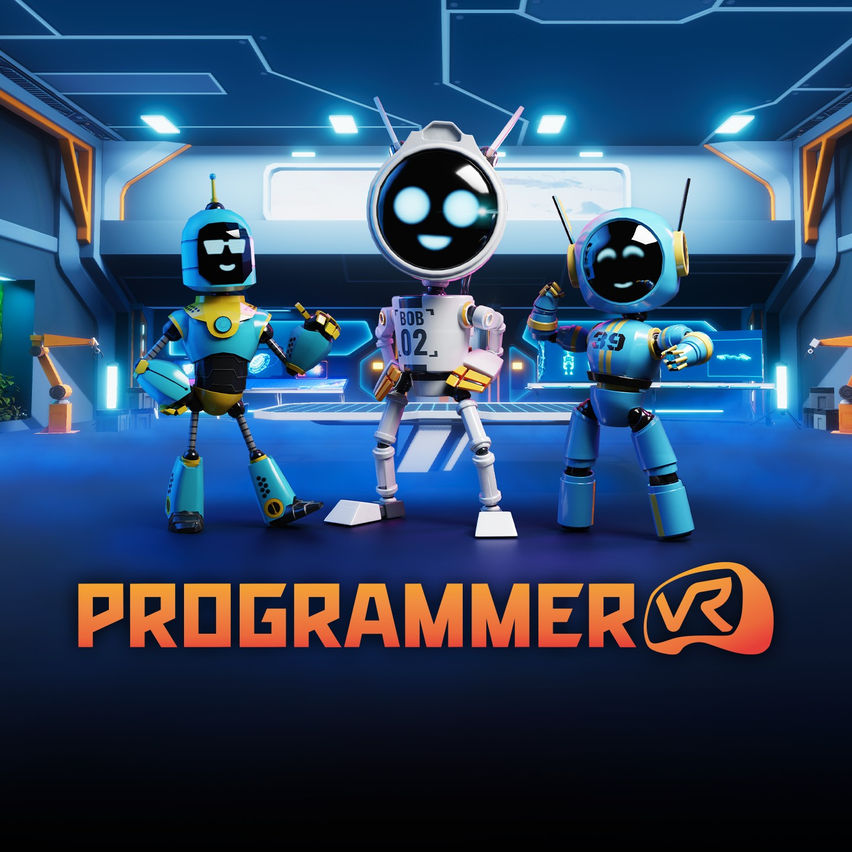
\includegraphics[width=0.8\textwidth]{pvr.jpeg}
\end{figure}

\textbf{ProgrammerVR}\footnote{\url{https://www.meta.com/experiences/programmer-vr/4987737161326497/}}
je virtuálna realita aplikácia určená pre výuku programovania.
Táto platforma ponúka možnosť programovať pomocou tvorby postupnosti príkazov priamo vo virtuálnej realite,
čím zvyšuje zážitok z učenia.
Obsahuje pripravenú sadu úloh na zoznámenie sa so základnými konceptmi programovania,
akými sú cykly a vetvenia.
Program je prístupný cez ekosystém Meta Quest,
čo znamená vysokú dostupnosť a relatívne jednoduché používanie.

\newpage

\section*{Snímky obrazovky z aplikácie}

\begin{figure}[H]
    \centering
    \begin{subfigure}[b]{0.49\textwidth}
        \centering
        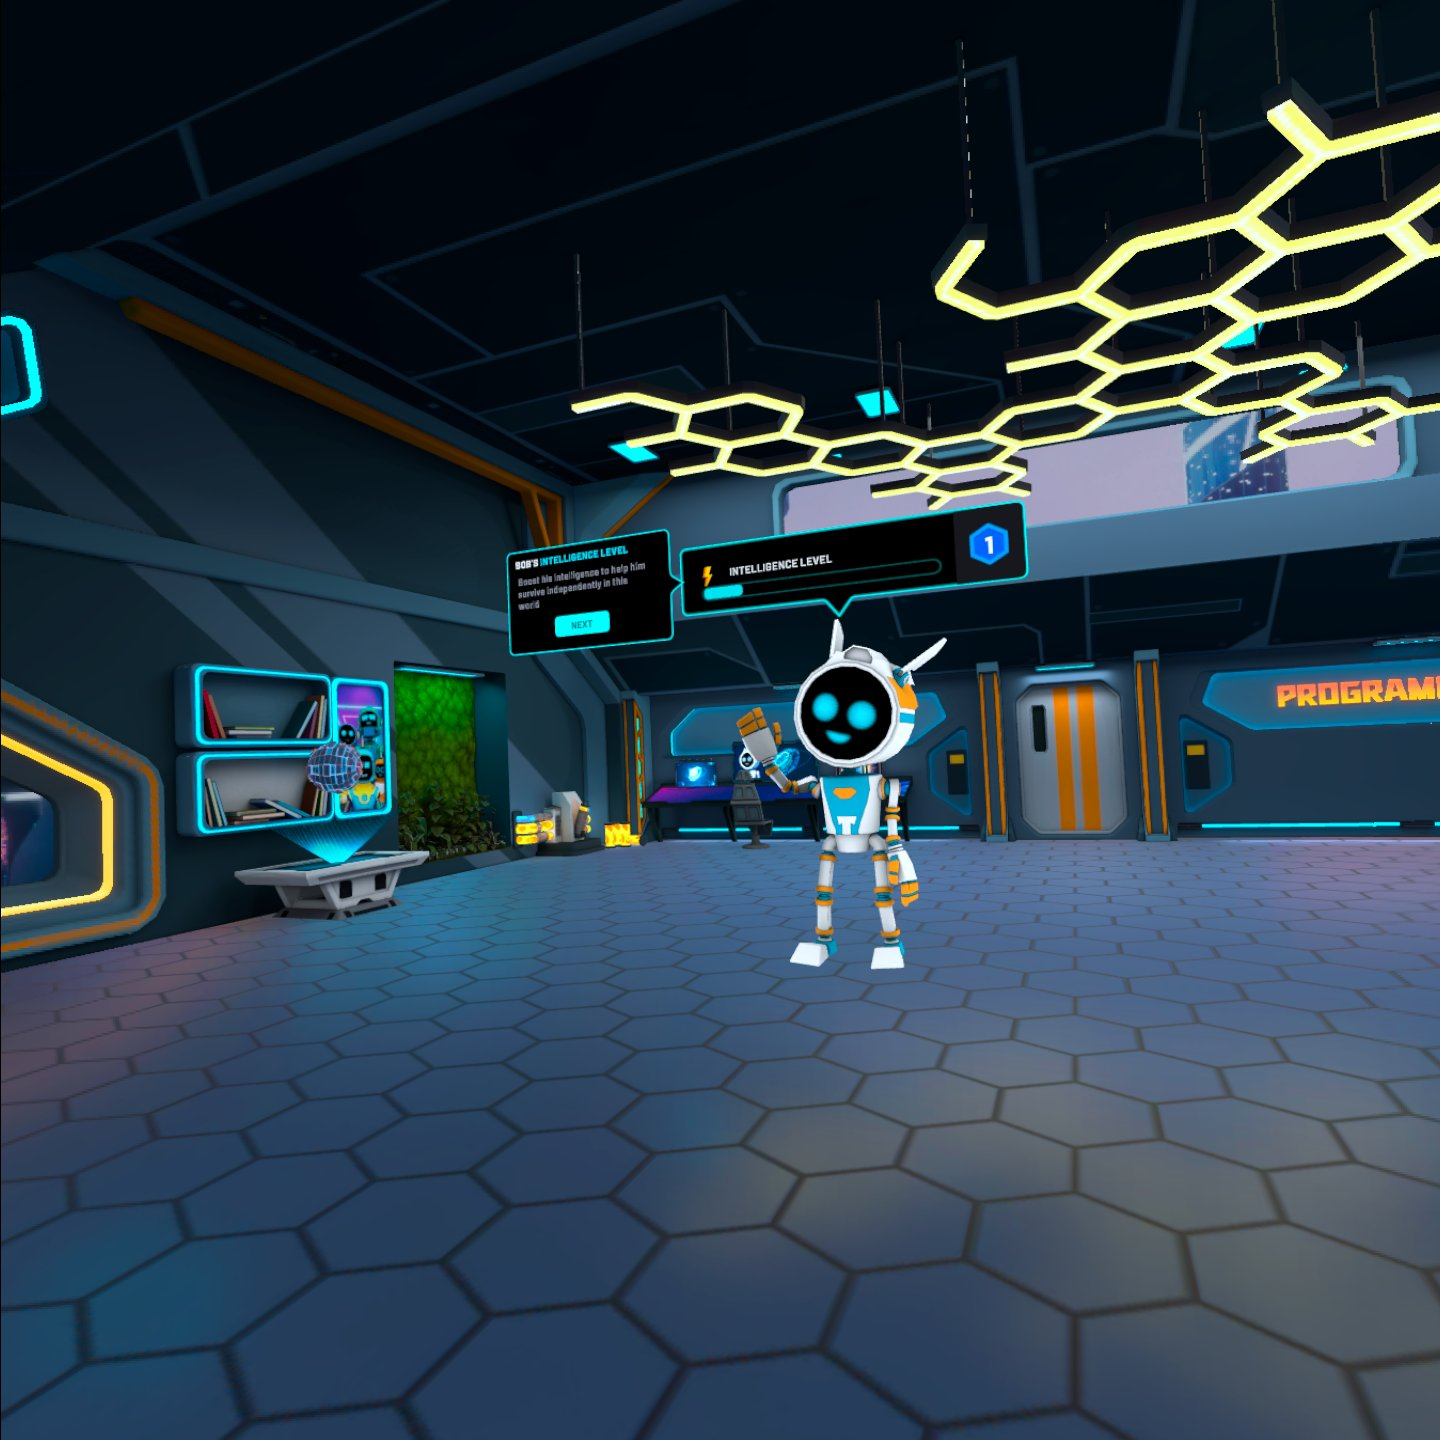
\includegraphics[width=\textwidth]{screen1.jpg}
    \end{subfigure}
    \begin{subfigure}[b]{0.49\textwidth}
        \centering
        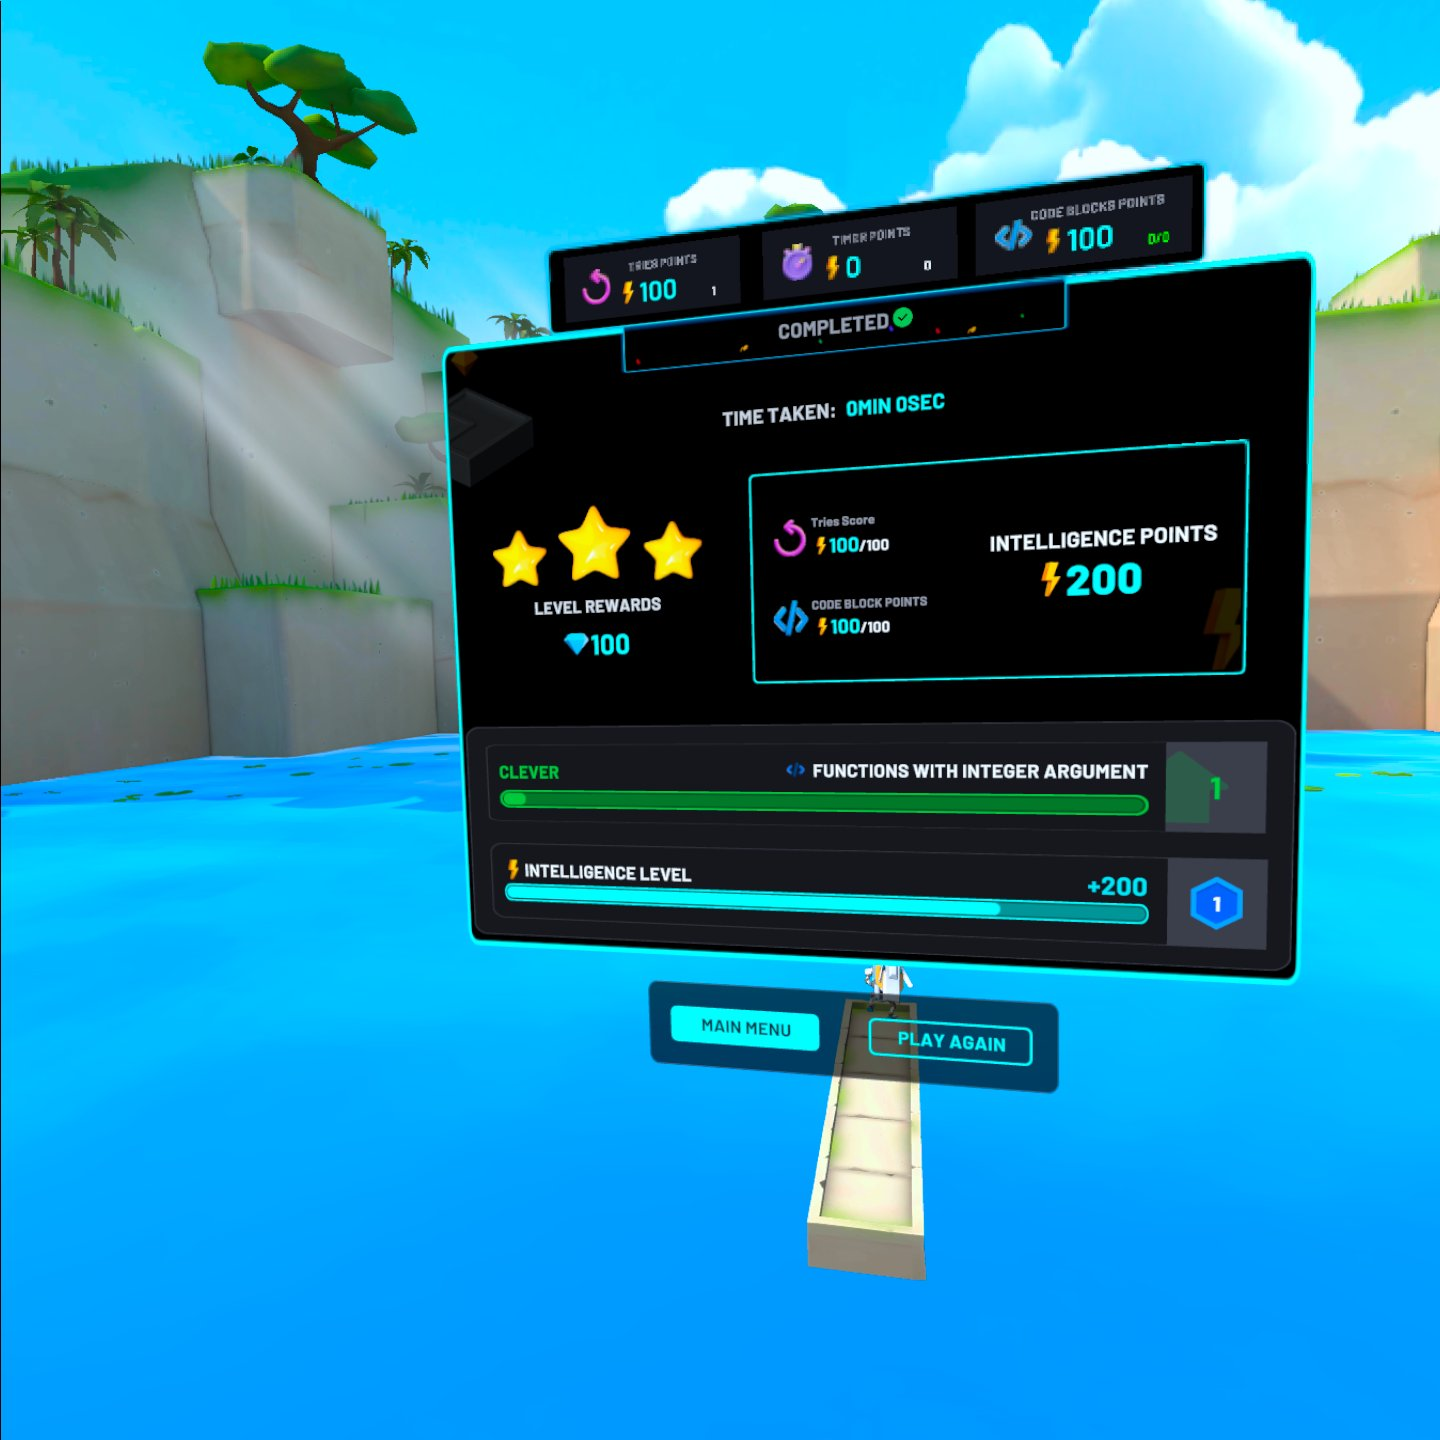
\includegraphics[width=\textwidth]{screen2.jpg}
    \end{subfigure}
    \begin{subfigure}[b]{0.49\textwidth}
        \centering
        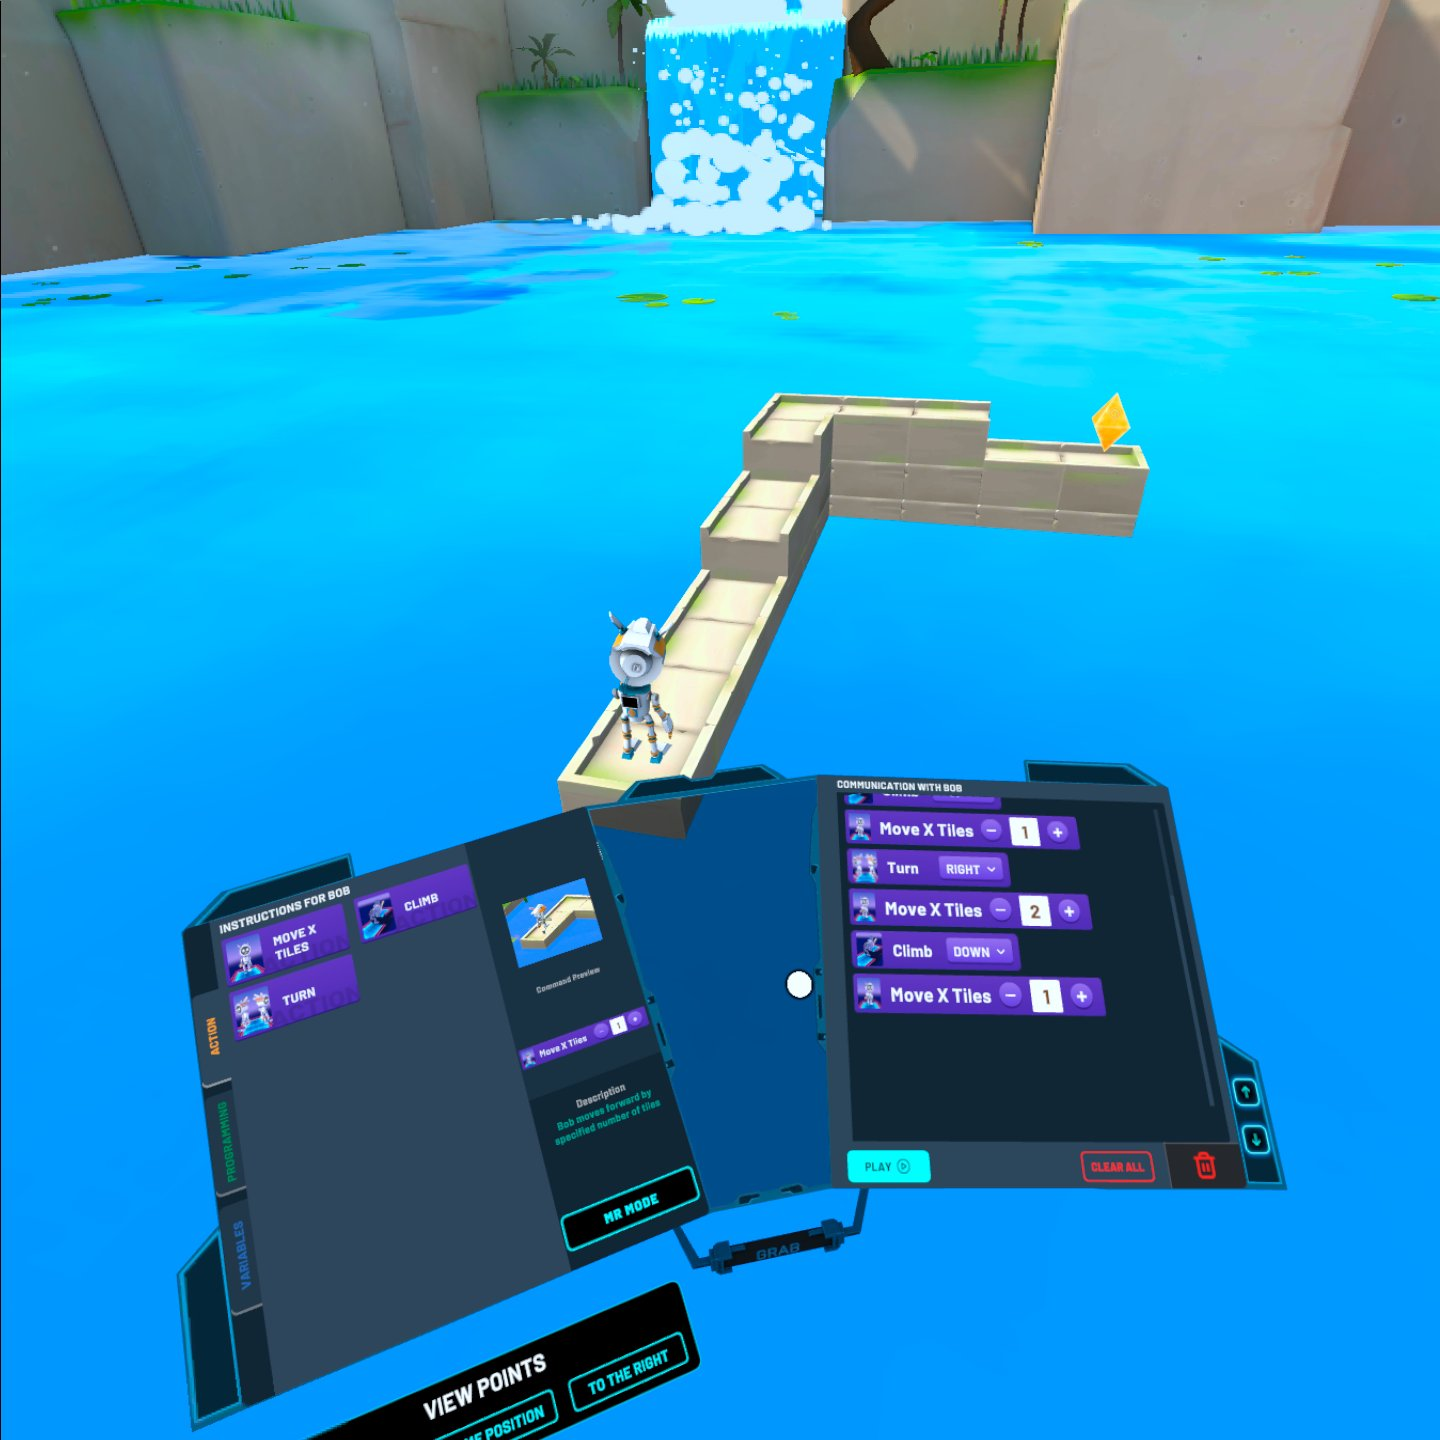
\includegraphics[width=\textwidth]{screen3.jpg}
    \end{subfigure}
    \begin{subfigure}[b]{0.49\textwidth}
        \centering
        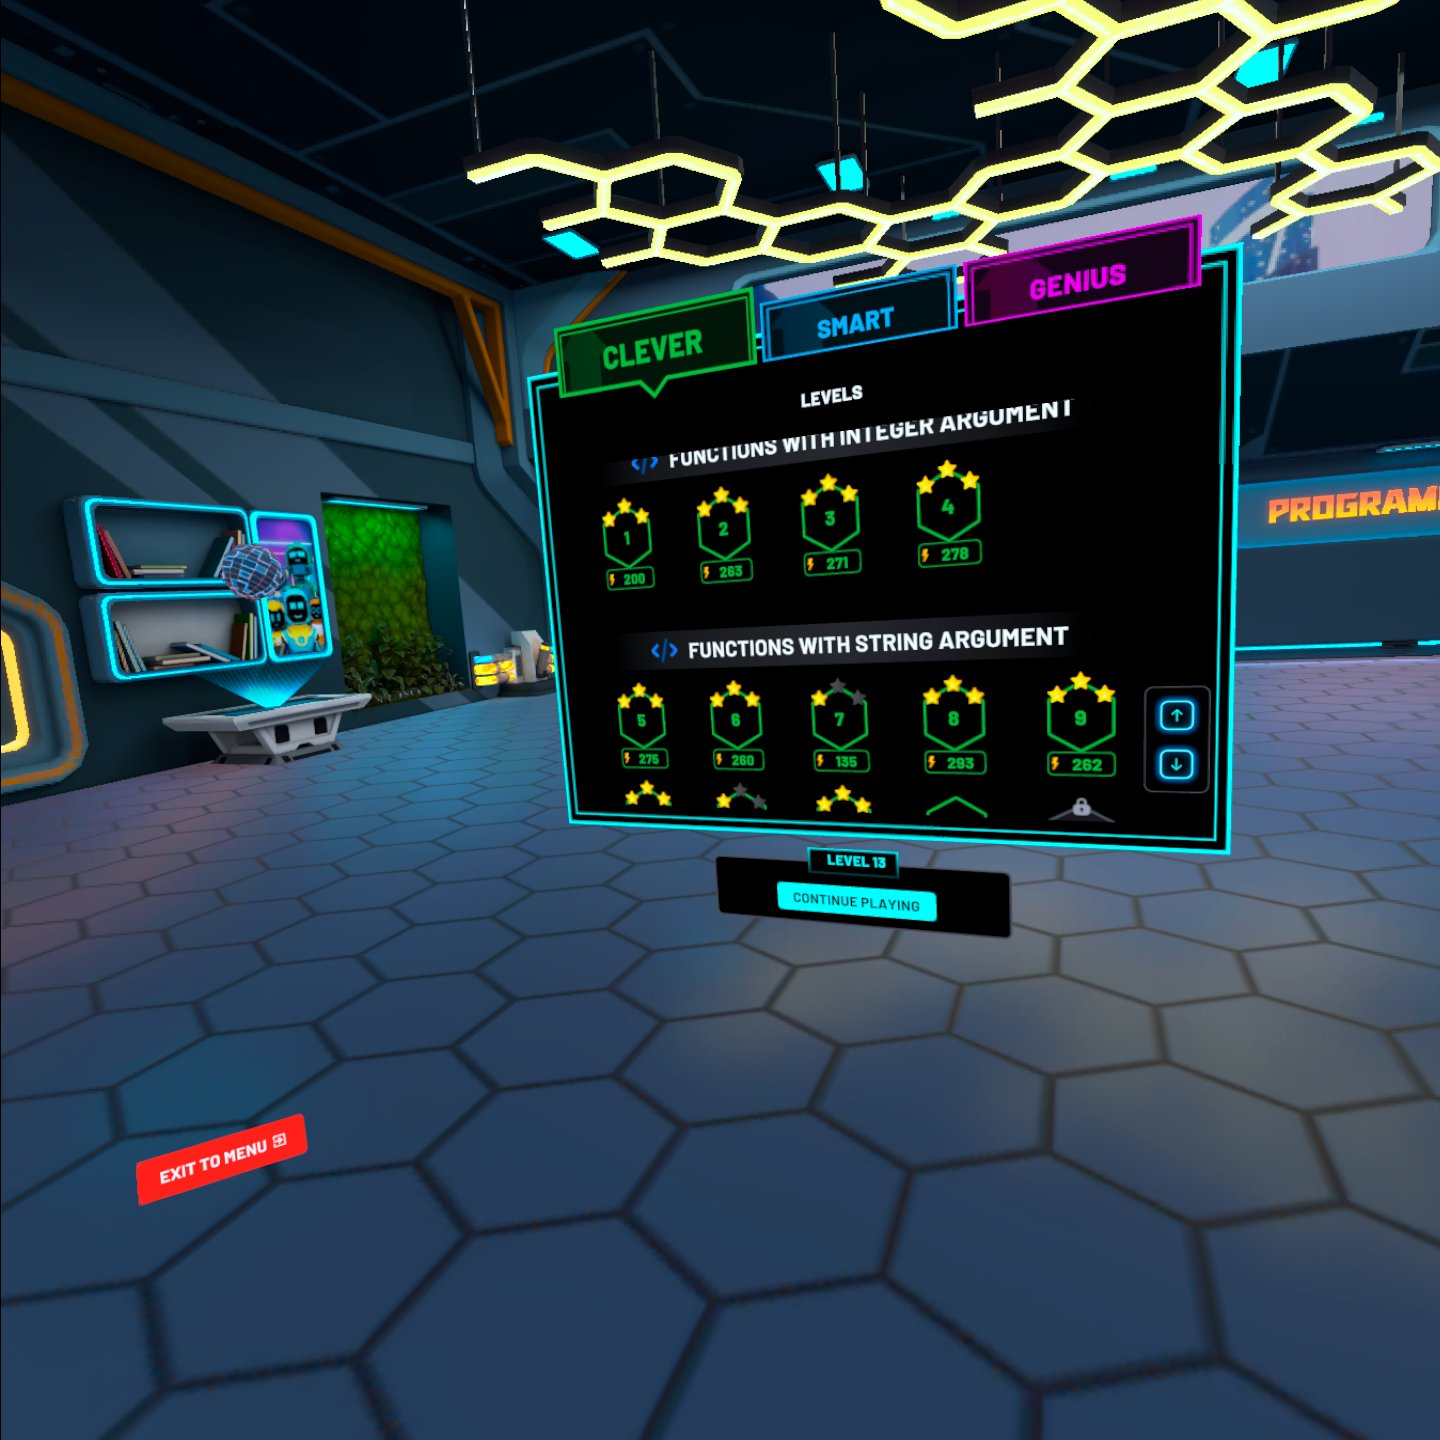
\includegraphics[width=\textwidth]{screen4.jpg}
    \end{subfigure}
\end{figure}

\newpage


\section{Charakteristika programu}
Program je komerčný produkt dostupný na platforme Meta Quest.
Pre používanie teda vyžaduje VR Headset od firmy Meta. Na ich platforme je následne dostupný
za cenu 19.99 \euro{} pre jedného používateľa. Ide o interaktívnu aplikáciu, kde používatelia vkladajú
príkazy a ich sekvencie pre úspešnú navigáciu robota cez prekážkovú dráhu.


Je určený predovšetkým pre študentov základných a stredných škôl,
ktorí sa chcú naučiť základy programovania a algoritmického myslenia.
Didaktickým cieľom aplikácie je uviesť žiakov do sveta programovania a informatiky
prostredníctvom interaktívnej, zábavnej a vizuálne príťažlivej formy.


\section{Edukačný pohľad}
ProgrammerVR poskytuje okamžitú spätnú väzbu na sekvenciu príkazov vytvorenú žiakom.
Aplikácia je navrhnutá pre individuálne aj skupinové použitie. V skupinovom móde môžu žiaci buď
súťažiť medzi sebou o najrýchlejšie vyriešenie zadania, alebo úlohy riešiť kolaboratívne.
Program využíva vizualizáciu vo VR prostredí na zvýšenie motivácie žiakov.


Obsah je prispôsobený začiatočníkom a pokrýva základy programovania bez potreby predchádzajúcich znalostí.
Aktuálne program obsahuje 75 hádaniek rozdelených do 3 úrovní podľa náročnosti.
Podľa dostupných informácií v súčasnosti nie je možné pridávať ani meniť úlohy.


\section{Odborná vhodnosť}
ProgrammerVR je navrhnutý tak, aby zodpovedal potrebám začiatočníkov v oblasti programovania,
čo zaručuje, že náročnosť aplikácie je primeraná veku a nemala by vyžadovať žiadne špeciálne znalosti
nad rámec študentov stredných škôl.


Program používa správnu terminológiu v oblasti informatiky.
Na prezentáciu využíva príbehové motívy a je zasadený do hernej situácie,
čo zvyšuje jeho edukatívnu hodnotu a angažovanosť študentov.
Vyučovanie prostredníctvom VR umožňuje zábavnú a interaktívnu formu učenia,
ktorá podporuje poznávací proces v rôznych fázach učenia. Vďaka dizajnu programu, v ktorom úlohy
začínajú od úplne jednoduchých, je možné ho zasadiť do vyučovania informatiky v ľubovoľnom štádiu
výučby na strednej škole.


\section{Pohľad používateľa}
ProgrammerVR je jednoduchý na ovládanie, interaktívny a ponúka atraktívny vizuálny a zvukový dizajn.
Aplikácia je stabilná a odolná voči chybám vo vstupe, čo znižuje frustráciu pri učení.
Počas testovania som nenarazil na žiadne bugy, príkazy sa vkladajú z dostupnej ponuky podobne ako napr.
v Scratchi. Takýto dizajn zaručuje dobrú odolnosť voči nečakaným zlým vstupom alebo preklepom.


Po stránke ovládateľnosti dodržiava štandardný spôsob ovládania VR aplikácií pomocou pohybových ovládačov.
Tento prístup je samozrejme radikálne iný od bežného používania myši a klávesnice.
Spôsob ovládania takýchto VR aplikácií sa snaží byť intuitívny, využíva metaforu chytania a presúvania
panelov a príkazov vo virtuálnom svete. Pre úspešné ovládanie je nutné zoznámiť sa s pohybovými ovládačmi
a ich tlačidlami. Na úchop sa napr. používa bočné tlačidlo. Aplikácia už ale má experimentálny režim,
v ktorom ju vieme ovládať čisto pomocou rúk, ktoré sú sledované kamerami. Rukami potom používateľ vykonáva
rôzne gestá a interaguje s predmetmi vo virtuálnom prostredí. Pred zaradením do vyučovania by sme určite
najskôr žiakov museli zaškoliť do základných princípov používania VR. Každopádne aplikácia dobre dodržiava
tieto princípy a teda pre niekoho so skúsenosťou s VR je veľmi jednoduchá na ovládanie.
Žiaľ, program v súčasnosti nie je dostupný v slovenskom jazyku.


\section{Technické vlastnosti}
Softvér vyžaduje VR zariadenie Meta Quest, ktorého cena začína na 300 \euro{}.
Školy, ktoré vlastnia takéto zariadenia patria skôr medzi výnimky, avšak populárnosť tejto technológie
aj v oblasti edukácie neustále rastie.


Samotná inštalácia programu je bezproblémová.
Program je dostupný priamo v zabudovanom obchode na týchto zariadeniach
a teda inštalácia prebieha podobne ako pri aplikáciách na smartfóne. Obsahuje zrozumiteľný
tutoriál a aj pomocníka s vysvetlivkami.
Úlohy sú v aplikácii rozdelené tematicky a zoradené podľa náročnosti, škola môže dodržať túto metodiku.


\section{Manažment výučby a hodnotenia žiakov}
Aplikácia zatiaľ neobsahuje rozsiahle nástroje pre manažment výučby alebo hodnotenia.
Neudržiava učiteľské záznamy o práci žiaka ani neponúka nástroje pre import alebo export dát.
Vývojári by mohli v budúcnosti zvážiť pridanie týchto funkcií na zlepšenie edukačnej hodnoty aplikácie.


Pre individuálne použitie ale obsahuje dostatok metód na sumarizáciu výsledkov.
Riešenia úloh sú hodnotené hviezdičkami, čo motivuje používateľa k iteratívnemu zlepšovaniu.
Žiak zároveň vidí počet svojich vyriešených úloh v jednotlivých kategóriách a jeho progres sa ukladá.
K riešeniu ďalších úloh sa teda môže kedykoľvek vrátiť. Sú tu zároveň rôzne rebríčky, kde môže svoj
výkon porovnávať s ostatnými používateľmi. Program využíva sieťovú komunikáciu v skupinovom režime
pri súťažení proti ostatným hráčom a kolaboratívnom riešení.


\end{document}

